\documentclass[11pt,a4paper]{article}

% ------------------------------------------------------------------ %
% Packages (chosen to compile cleanly with tectonic / XeTeX)          %
% ------------------------------------------------------------------ %
\usepackage[margin=1in]{geometry}
\usepackage{graphicx}
\usepackage{booktabs}
\usepackage{longtable}
\usepackage{array}
\usepackage[table]{xcolor}
\usepackage{enumitem}
\usepackage{tikz}
\usetikzlibrary{positioning,arrows.meta,shapes.geometric,fit,backgrounds,calc}
\usepackage{caption}
\usepackage{amsmath}
\usepackage{float}
\usepackage{listings}
\usepackage{underscore} % lets bare _ print in text/tables (many snake_case tokens)
\usepackage[hidelinks]{hyperref}

% ------------------------------------------------------------------ %
% Status colours + macros                                             %
% ------------------------------------------------------------------ %
\definecolor{cok}{HTML}{1B7F3B}     % green   - complete / verified / implemented
\definecolor{cpart}{HTML}{B26B00}   % orange  - partial / pending
\definecolor{cmiss}{HTML}{B00020}   % red     - missing / blocked
\definecolor{cnv}{HTML}{5A5A5A}     % gray    - not verified
\definecolor{cplan}{HTML}{123A5E}   % blue    - planned
\definecolor{hdr}{HTML}{123A5E}

\newcommand{\stImpl}{\textcolor{cok}{\textbf{IMPLEMENTED}}}
\newcommand{\stV}{\textcolor{cok}{\textbf{VERIFIED}}}
\newcommand{\stP}{\textcolor{cpart}{\textbf{PARTIAL}}}
\newcommand{\stPend}{\textcolor{cpart}{\textbf{PENDING}}}
\newcommand{\stB}{\textcolor{cmiss}{\textbf{BLOCKED}}}
\newcommand{\stPlan}{\textcolor{cplan}{\textbf{PLANNED}}}
\newcommand{\stNV}{\textcolor{cnv}{\textbf{NOT VERIFIED}}}
\newcommand{\code}[1]{\texttt{\small #1}}

% Prefer loose spacing over text bleeding into the margin (dense snake_case/slash tokens),
% and silence cosmetic underfull-hbox noise in narrow longtable columns.
\sloppy
\setlength{\emergencystretch}{3em}
\hbadness=10000

\lstset{
  basicstyle=\ttfamily\footnotesize,
  breaklines=true,
  frame=single,
  columns=fullflexible,
  keepspaces=true,
  showstringspaces=false,
  xleftmargin=0.5em
}

% TikZ node styles
\tikzset{
  box/.style={rectangle, rounded corners=2pt, draw=hdr, fill=blue!5, thick,
              text width=2.5cm, align=center, minimum height=0.9cm, font=\small},
  agent/.style={rectangle, rounded corners=2pt, draw=cok, fill=green!6, thick,
              text width=2.5cm, align=center, minimum height=0.8cm, font=\small},
  warn/.style={rectangle, rounded corners=2pt, draw=cpart, fill=orange!8, thick,
               text width=2.5cm, align=center, minimum height=0.8cm, font=\small},
  flow/.style={-{Stealth[length=2.2mm]}, thick, draw=hdr}
}

\hypersetup{
  pdftitle={SuryaGrid AI: Execution Plan - Substation-Driven Forecasting and DSM Workflow},
  pdfauthor={SuryaGrid Project Team}
}

% ------------------------------------------------------------------ %
\begin{document}

\begin{titlepage}
\centering
\vspace*{2.2cm}
{\Huge\bfseries SuryaGrid AI\par}
\vspace{0.5cm}
{\LARGE Execution Plan: Substation-Driven Forecasting and DSM Workflow\par}
\vspace{0.8cm}
{\large Bengaluru / Karnataka / India Solar-Grid Forecasting\\ and DSM Multi-Agent Platform\par}
\vspace{2cm}
{\large\itshape Technical Execution Plan and Workflow Document\par}
\vspace{1.5cm}
\begin{tabular}{rl}
\textbf{Prepared by:} & SuryaGrid Project Team\\[4pt]
\textbf{Date:} & 7 July 2026\\[4pt]
\textbf{Baseline commit:} & \code{5bed3cd} (substation-driven workflow foundation)\\[4pt]
\textbf{Scope:} & Next development phase; planning only (no app code changed)\\[4pt]
\textbf{Repositories:} & DBIT-Banglore/SuryaGrid, lekhanpro/SuryaGrid\\
\end{tabular}
\vfill
{\footnotesize This is a planning document. Every \stImpl\ item is backed by a repository file,
model card, test, or command output verified this session. Items needing data the repository
does not contain are marked \stB\ with the required official source. Nothing is fabricated;
un-run or absent capabilities are marked \stPlan, \stPend, or \stNV.\par}
\end{titlepage}

\tableofcontents
\newpage

% ================================================================== %
\section{Executive Summary}
\addcontentsline{toc}{section}{Executive Summary}
SuryaGrid AI is an architecturally complete, partially data-complete prototype. The FastAPI
backend exposes \textbf{61} \code{/api/v1} operations and passes \textbf{118} tests
(\code{ruff check} clean); the Next.js~14 frontend builds (16 static routes). Real-data models
are trained and carry cards: solar irradiance $R^2=0.956$, cloud-risk $F_1=0.67$ / AUC$=0.90$,
DSM-breach $F_1=0.79$ (Open-Meteo Bengaluru), plus a Kaggle Bengaluru irradiance model
$R^2=0.920$ and cloud model $F_1=0.847$. 344 substations are ingested from OpenStreetMap
(\textbf{capacity 0\%, voltage 41\%}; capacity is never fabricated).

As of commit \code{5bed3cd} the \textbf{substation-driven workflow foundation is implemented}:
a \code{SubstationContext} object, a context service over the real parquet, an orchestrator
agent, five endpoints, honest DSM blocking, \code{agent\_trace} / \code{calculation\_trace}, and
a frontend \code{SubstationWorkflowPanel} wired into the Locations and DSM pages, covered by 15
tests. \textbf{The remaining gap} is dashboard-wide substation context: the main dashboard still
runs from a hardcoded location preset list, so this phase makes the selected \code{substation\_id}
the single active context for \emph{every} dashboard card (weather, solar, cloud, generation
timeline, DSM, source/limitation, agent-trace), adds a shared/persisted selection, reconciles the
database-backed \code{/substations} list with the parquet-backed \code{/substations/catalog}, and
hardens source-trace and missing-data surfacing across the UI.

\textbf{Why substation-driven context is needed.} A dropdown that only changes display text is
cosmetic. Grid behaviour (irradiance at the substation coordinates, cloud risk, generation,
deviation risk) is location-specific: the selection must change the \emph{actual agent input
context}, and every value must remain traceable with missing fields explicit. \textbf{Expected
outcome:} selecting a substation refreshes all panels with values computed for that substation's
coordinates and provenance; DSM output lists enabled vs blocked calculations honestly (no
rupee/capacity/load fabrication); responses always carry an agent trace and a calculation trace;
tests and the frontend build pass.

% ================================================================== %
\section{Current Verified Baseline}
Table~\ref{tab:baseline} is derived from the repository, model cards,
\code{report\_evidence\_matrix.md}, \code{substation\_data\_quality\_report.md}, and the
\code{5bed3cd} verification. Nothing is asserted beyond these sources.

\begin{footnotesize}
\begin{longtable}{@{}p{2.4cm}p{4.4cm}p{4.0cm}p{3.5cm}@{}}
\caption{Current verified baseline (Table 1).}\label{tab:baseline}\\
\toprule
\textbf{Area} & \textbf{Current verified status} & \textbf{Evidence} & \textbf{Limitation / next action}\\
\midrule
\endfirsthead
\toprule
\textbf{Area} & \textbf{Current verified status} & \textbf{Evidence} & \textbf{Limitation / next action}\\
\midrule
\endhead
\bottomrule
\endfoot
Backend API & \stImpl\ 61 \code{/api/v1} ops; 118 tests pass & route introspection; \code{pytest -q} & keep parity as UI wires in\\
Substation workflow (backend) & \stImpl\ context + orchestrator + 5 endpoints (\code{5bed3cd}) & \code{schemas/}, \code{services/}, \code{agents/}, \code{api/} files & combined only; per-card UI \stPlan\\
Agents & \stImpl\ 16 platform agents + 7-step orchestrator & \code{agents/*}; \code{agent\_trace} & weather live-fetch degrades to clear-sky\\
ML models & \stImpl\ 3 Open-Meteo + 2 Kaggle prod; \stP\ PV/load non-prod; RL untrained & \code{models/metadata/*} cards & PV/load REAL\_INDIA (domain shift)\\
ML datasets & \stImpl\ parquet + manifests present & \code{data/ml/*.parquet} & large parquets gitignored (reproducible)\\
Data sources & \stP\ Open-Meteo + OSM live; NASA cross-check only; Kaggle used & \code{data\_sources/}, registries & NASA live + SLDC/CEA \stPlan\\
Substation data & \stImpl\ 344 OSM rows committed; capacity 0\%, voltage 41\% & \code{bengaluru\_substations\_cleaned.parquet} & \stB\ needs KPTCL/BESCOM capacity\\
DSM & \stP\ framework + ML breach; no rupee values & \code{predict\_dsm}; \code{emits\_rupee\_values=false} & \stB\ needs KERC/CERC tariff order\\
Frontend & \stImpl\ builds (16 routes); panel on Locations+DSM & \code{npm run build}; \code{SubstationWorkflowPanel.tsx} & dashboard uses hardcoded preset \stPlan\\
Deployment & \stP\ single-instance docker-compose+nginx live (HTTP) & evidence matrix A1--A6 & DB record\_counts$=0$; ECS code-only\\
Lint & \stImpl\ \code{ruff check} clean; \stP\ format-check 5 pre-existing files & verified this session & optional format-only follow-up\\
\end{longtable}
\end{footnotesize}

\noindent\textbf{Must not be claimed (tracked \stB):} substation capacity (MVA), metered
Karnataka/feeder load, official parsed KERC/CERC rupee tariff rates, local Bengaluru PV generation
truth, deployed AWS ECS stack.

% ================================================================== %
\section{Problem Statement}
Substations exist in the system (344 real OSM rows via \code{/substations/catalog}) and the
backing endpoints exist (\code{5bed3cd}). The gap is that the selected substation is not yet the
active context across the whole product surface:
\begin{itemize}[leftmargin=1.4em,itemsep=1pt]
  \item The main dashboard (\code{frontend/app/dashboard/page.tsx}) drives its cards from a
        hardcoded \code{LOCATIONS} preset array and \code{predictSite("primary-site", ...)}, not
        from a substation.
  \item The substation dropdown currently lives only inside \code{SubstationWorkflowPanel} on the
        Locations and DSM pages; it does not update the separate weather / solar / cloud /
        timeline / DSM / source / agent-trace cards, and there is no shared selection.
  \item The database-backed \code{/substations} list and the parquet-backed
        \code{/substations/catalog} can disagree (hosted DB \code{record\_counts}$=0$ returns an
        empty list, while the catalog returns 344).
\end{itemize}
\noindent\textbf{Requirement:} the dropdown must change the \emph{actual agent input context}. The
selected \code{substation\_id} must flow to the backend, become a \code{SubstationContext}, reach
every agent, the DSM engine, and the orchestrator, and refresh every relevant panel with source
trace, agent trace, and explicit missing/blocked handling.

% ================================================================== %
\section{Target Architecture}
Figure~\ref{fig:flow} shows the request flow from selection to dashboard;
Figure~\ref{fig:arch} shows the backend architecture with implemented (\stImpl) versus planned
(\stPlan) elements.

\begin{figure}[H]
\centering
\resizebox{\textwidth}{!}{%
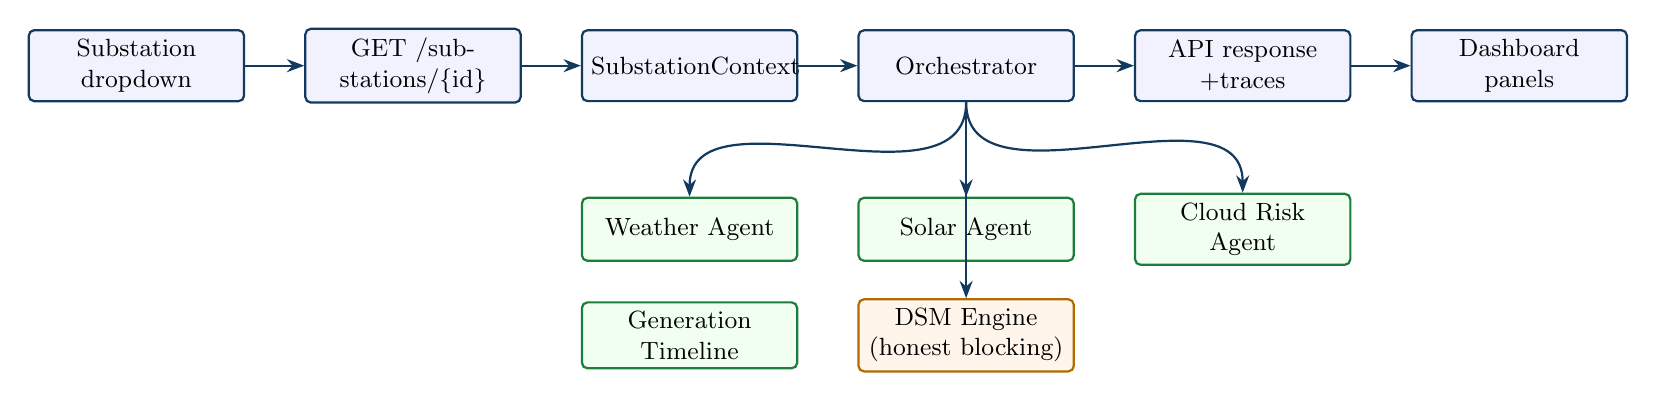
\begin{tikzpicture}[node distance=0.55cm and 0.75cm]
\node[box] (dd) {Substation dropdown};
\node[box, right=of dd] (get) {GET /substations/\{id\}};
\node[box, right=of get] (ctx) {SubstationContext};
\node[box, right=of ctx] (orc) {Orchestrator};
\node[box, right=of orc] (resp) {API response\\+traces};
\node[box, right=of resp] (ui) {Dashboard panels};
\node[agent, below=1.2cm of ctx] (w) {Weather Agent};
\node[agent, right=of w] (s) {Solar Agent};
\node[agent, right=of s] (k) {Cloud Risk Agent};
\node[agent, below=0.5cm of w] (g) {Generation Timeline};
\node[warn, right=of g] (x) {DSM Engine\\(honest blocking)};
\draw[flow] (dd)--(get); \draw[flow] (get)--(ctx); \draw[flow] (ctx)--(orc);
\draw[flow] (orc)--(resp); \draw[flow] (resp)--(ui);
\draw[flow] (orc.south) to[out=-90,in=90] (w.north);
\draw[flow] (orc.south) to[out=-90,in=90] (s.north);
\draw[flow] (orc.south) to[out=-90,in=90] (k.north);
\draw[flow] (orc.south) to[out=-90,in=90] (x.north);
\end{tikzpicture}}
\caption{Selection $\rightarrow$ context $\rightarrow$ agents $\rightarrow$ dashboard (Figure 1).
Blue = request path; green = agents; orange = DSM with honest blocking.}
\label{fig:flow}
\end{figure}

\begin{figure}[H]
\centering
\resizebox{0.96\textwidth}{!}{%
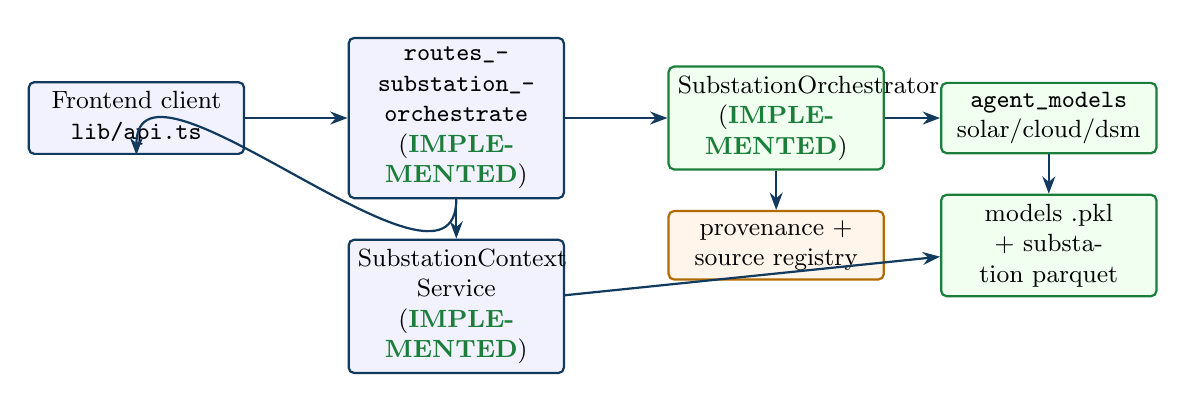
\begin{tikzpicture}[node distance=0.5cm and 0.7cm]
\node[box] (client) {Frontend client\\\code{lib/api.ts}};
\node[box, right=1.3cm of client] (r1) {\code{routes\_substation\_} \code{orchestrate} (\stImpl)};
\node[agent, right=1.3cm of r1] (orc) {SubstationOrchestrator (\stImpl)};
\node[agent, right=of orc] (am) {\code{agent\_models} solar/cloud/dsm};
\node[box, below=of r1] (ctx) {SubstationContext Service (\stImpl)};
\node[agent, below=of am] (ml) {models .pkl + substation parquet};
\node[warn, below=of orc] (pr) {provenance + source registry};
\draw[flow] (client)--(r1); \draw[flow] (r1)--(orc); \draw[flow] (orc)--(am);
\draw[flow] (r1)--(ctx); \draw[flow] (ctx)--(ml); \draw[flow] (am)--(ml);
\draw[flow] (orc)--(pr); \draw[flow] (r1.south) to[out=-90,in=90] (client.south);
\end{tikzpicture}}
\caption{Backend architecture (Figure 2). All shown blocks are \stImpl\ at \code{5bed3cd};
the frontend consumption of these across all dashboard cards is \stPlan.}
\label{fig:arch}
\end{figure}

% ================================================================== %
\section{SubstationContext Specification}
Canonical object (\code{backend/app/schemas/substation\_context.py}, \stImpl). Built by
\code{SubstationContextService.get\_context()}, which coerces \code{None} / \code{NaN} /
\code{"nan"/"none"/"null"/""} to \code{null}.

\begin{lstlisting}
substation_id, name, latitude, longitude          # identity/geography (always present)
operator          # 147/344 present, else null
voltage_kv        # 141/344 present, else null
capacity_mva      # 0/344 present -> ALWAYS null (never fabricated)
district          # 0/344 present -> ALWAYS null
state, source, source_url, reliability_score, missing_fields, data_geography, ingestion_time
display_label, distance_from_site_km, nearest_weather_location
weather_source    # "Open-Meteo @ (lat,lon) [REAL_COORDINATE_BASED]"
solar_source      # "solar_forecast_model.pkl [REAL_BENGALURU]"
tariff_region     # "Karnataka (KERC)"
source_status     # REAL_BENGALURU | REAL_KARNATAKA
capacity_status   # NOT_AVAILABLE (capacity null)
voltage_status    # source_status | NOT_AVAILABLE
load_data_status  # NOT_AVAILABLE
tariff_status     # NEEDS_OFFICIAL_SOURCE
limitation_notes  # human-readable honesty notes
\end{lstlisting}

\noindent\textbf{Rules (enforced):} missing \code{capacity\_mva} stays \code{null}
($\rightarrow$ \code{capacity\_status=NOT\_AVAILABLE}); missing \code{voltage\_kv} stays
\code{null} ($\rightarrow$ \code{voltage\_status=NOT\_AVAILABLE}); load is \code{NOT\_AVAILABLE};
tariff is \code{NEEDS\_OFFICIAL\_SOURCE}; no value is fabricated.

% ================================================================== %
\section{Detailed Agent Workflow}
Implemented in \code{SubstationOrchestrator.run()} (\stImpl). Every step appends to
\code{agent\_trace}; every number records its formula + provenance in \code{calculation\_trace}.

\begin{footnotesize}
\begin{longtable}{@{}p{0.4cm}p{2.3cm}p{3.4cm}p{3.0cm}p{3.6cm}@{}}
\caption{Substation-driven agent workflow (Table 2).}\label{tab:workflow}\\
\toprule
\textbf{\#} & \textbf{Agent/Service} & \textbf{Input $\rightarrow$ processing} & \textbf{Output} & \textbf{Source trace / missing-data behaviour}\\
\midrule
\endfirsthead
\toprule
\textbf{\#} & \textbf{Agent/Service} & \textbf{Input $\rightarrow$ processing} & \textbf{Output} & \textbf{Source trace / missing-data behaviour}\\
\midrule
\endhead
\bottomrule
\endfoot
1 & Frontend selection & user click $\rightarrow$ substation\_id & request w/ substation\_id & disabled until catalog loads\\
2 & Context Service & substation\_id $\rightarrow$ load parquet, coerce, statuses & SubstationContext & REAL\_BENGALURU/KARNATAKA; unknown id $\rightarrow$ 404; missing $\rightarrow$ null+status\\
3 & Weather Agent & lat/lon $\rightarrow$ Open-Meteo @ coords & hourly weather + GHI & REAL\_COORDINATE\_BASED; net fail $\rightarrow$ pvlib clear-sky (labelled), never synthetic\\
4 & Solar Agent & context+weather+model $\rightarrow$ \code{predict\_solar} & irradiance (+est. PV if capacity) & REAL\_BENGALURU; model missing $\rightarrow$ NOT\_AVAILABLE\\
5 & Cloud Risk Agent & weather features $\rightarrow$ \code{predict\_cloud} & P(kt$<$0.5) drop risk & REAL\_BENGALURU; model missing $\rightarrow$ NOT\_AVAILABLE\\
6 & Generation Timeline & weather+solar+cloud+substation & hourly rows (each carries substation\_id) & ESTIMATED\_FROM\_IRRADIANCE; no capacity $\rightarrow$ MW null\\
7 & DSM Engine & context+timeline+status $\rightarrow$ \code{predict\_dsm}+gating & recommendation + blocked calcs & NEEDS\_OFFICIAL\_SOURCE; capacity/load/tariff missing $\rightarrow$ block+reason\\
8 & Orchestrator & all outputs $\rightarrow$ assemble & response + agent\_trace + calculation\_trace & ESTIMATED\_FROM\_REAL; degraded steps flagged\\
9 & Frontend render & response $\rightarrow$ update panels & refreshed dashboard & show warnings for missing/blocked\\
\end{longtable}
\end{footnotesize}

% ================================================================== %
\section{API Execution Plan}
Base \code{/api/v1}; envelope \code{\{success, message, data, timestamp\}}.

\begin{footnotesize}
\begin{longtable}{@{}p{3.5cm}p{1.6cm}p{4.0cm}p{4.4cm}@{}}
\caption{API endpoints: status and contract (Table 3).}\label{tab:api}\\
\toprule
\textbf{Endpoint} & \textbf{Status} & \textbf{Request $\rightarrow$ response (data)} & \textbf{Consumer / acceptance}\\
\midrule
\endfirsthead
\toprule
\textbf{Endpoint} & \textbf{Status} & \textbf{Request $\rightarrow$ response} & \textbf{Consumer / acceptance}\\
\midrule
\endhead
\bottomrule
\endfoot
GET \code{/substations} & \stImpl\ (DB) & \code{?limit} $\rightarrow$ DB rows (may be empty) & Locations table; list or explicit empty state\\
GET \code{/substations/catalog} & \stImpl & \code{?limit} $\rightarrow$ 344 \{id, display\_label, coords, voltage, reliability\} & Dropdown; loads 344\\
GET \code{/substations/\{id\}} & \stImpl & path id $\rightarrow$ full SubstationContext (404 if unknown) & Detail card; missing null\\
POST \code{/orchestrate/substation} & \stImpl & \{substation\_id, site\_capacity\_mw?, scheduled\_generation\_mw?, forecast\_horizon\_hours, use\_live\_weather\} $\rightarrow$ substation, trace, timeline, DSM, sources, limitations & Dashboard refresh; 7-step trace; \code{is\_synthetic=false}\\
POST \code{/dsm/forecast} & \stImpl & same body $\rightarrow$ dsm\_forecast (blocked calcs, no rupees)+trace & DSM panel; \code{emits\_rupee\_values=false}\\
GET \code{/generation/timeline} & \stImpl & \code{?substation\_id\&site\_capacity\_mw\&horizon\&allow\_estimated} $\rightarrow$ timeline, summary, weather, trace & Timeline component; rows carry substation\_id\\
\code{/substations} $\leftrightarrow$ \code{/catalog} reconcile & \stPlan & delegate UI to catalog or seed DB from parquet & one authoritative list on host\\
\end{longtable}
\end{footnotesize}

\noindent No new endpoints are strictly required; the only \stPlan\ API work is reconciling the DB
list with the parquet catalog so the dropdown is never empty on the hosted deployment.

% ================================================================== %
\section{Frontend Execution Plan}
Verified components: \code{ModelProvenancePanel}, \code{OfflineBanner},
\code{SubstationWorkflowPanel} (new), \code{cards/\{MetricCard,PenaltyStatusCard\}},
\code{charts/\{DeviationBar,MiniTimeline\}}, \code{svg/\{SolarPanel3D,RiskGauge3D,EnergyFlow3D\}}.
The dashboard currently uses a hardcoded \code{LOCATIONS} array.

\begin{footnotesize}
\begin{longtable}{@{}p{3.0cm}p{3.4cm}p{3.4cm}p{3.6cm}@{}}
\caption{Frontend changes (Table 4).}\label{tab:fe}\\
\toprule
\textbf{Component / page} & \textbf{Current behaviour} & \textbf{Required change} & \textbf{Endpoint / acceptance}\\
\midrule
\endfirsthead
\toprule
\textbf{Component / page} & \textbf{Current behaviour} & \textbf{Required change} & \textbf{Endpoint / acceptance}\\
\midrule
\endhead
\bottomrule
\endfoot
\code{lib/api.ts} & \stImpl\ catalog/context/orchestrate/dsm/timeline fns & reuse; shared fetch on selection & no mock in real mode\\
Substation dropdown & in panel on 2 pages & promote to shared selector (store/query param) & \code{/substations/catalog}; persists across pages\\
\code{app/dashboard/page.tsx} & hardcoded LOCATIONS + predictSite & add selector; drive cards from orchestrate & \code{/orchestrate/substation}; selecting refreshes\\
Detail / weather / solar / cloud cards & preset-driven / in panel & bind to orchestrate response & selected coords + provenance shown\\
Generation timeline (\code{MiniTimeline}) & \code{getTimeline(...)} & bind to \code{/generation/timeline} & rows carry substation\_id\\
DSM panel & in panel (dsm page) & dedicated dashboard card & blocked calcs + no rupees\\
Source/limitation + agent-trace panels & in panel & dashboard-wide panels & provenance + 7-step trace always visible\\
\end{longtable}
\end{footnotesize}

\noindent\textbf{Guardrail:} no redesign; reuse \code{glass-card}/\code{input-field}/
\code{btn-primary}; never render mock data when the backend is reachable; keep the
\code{OfflineBanner} behaviour.

% ================================================================== %
\section{DSM Engine Data Usage}
DSM step: \code{SubstationOrchestrator.\_build\_dsm\_forecast} + \code{agent\_models.predict\_dsm}
(\stImpl). \textbf{Input:} selected\_substation (context), generation\_timeline, solar\_forecast,
cloud\_risk, load\_data\_status, tariff\_source\_status, capacity\_status, voltage\_status,
source\_trace. \textbf{Output:} recommendation, action, risk/deviation\_band, confidence, fields
used (\code{context\_inputs\_used}), fields missing, calculations enabled, calculations blocked,
reason, limitation notes.

\begin{table}[H]\centering\footnotesize
\caption{Blocked-calculation rules (enforced) (Table 5).}\label{tab:dsm}
\begin{tabular}{@{}p{4.6cm}p{4.4cm}p{4.6cm}@{}}
\toprule
\textbf{Condition} & \textbf{Blocked calculation} & \textbf{Status flag}\\
\midrule
\code{capacity\_mva} missing (always, OSM) & \code{substation\_loading\_percent} & \code{capacity\_status=NOT\_AVAILABLE}\\
load data missing & \code{load\_following\_optimisation} & \code{load\_data\_status=NOT\_AVAILABLE}\\
official tariff missing & \code{dsm\_rupee\_charge} (settlement/savings) & \code{tariff\_status=NEEDS\_OFFICIAL\_SOURCE}; \code{emits\_rupee\_values=false}\\
PV generation unavailable & mark generation ESTIMATED & \code{actual\_generation\_available=false}\\
\code{voltage\_kv} missing & \code{voltage\_band\_optimisation} & \code{voltage\_status=NOT\_AVAILABLE}\\
\bottomrule
\end{tabular}
\end{table}

% ================================================================== %
\section{Generation Timeline and Trace Design}
\textbf{Timeline rows} (\stImpl; \stPlan\ items marked): \code{timestamp}, \code{substation\_id},
\code{substation\_label} (\stPlan\ explicit \code{substation\_name}), weather features
(\code{clearsky\_ghi\_wm2}, \code{observed\_ghi\_wm2}; \stPlan\ per-row temp/cloud),
\code{forecast\_ghi\_wm2}, \code{estimated\_generation\_mw} (if capacity; else null),
\code{cloud\_drop\_risk}, \stPlan\ \code{confidence\_components}, \code{data\_sources},
\code{limitations}. Rule: no actual generation $\rightarrow$
\code{generation\_type=ESTIMATED\_FROM\_IRRADIANCE}, \code{actual\_generation\_available=false}.

\medskip
\noindent\textbf{Traces.} \code{agent\_trace[]} carries \code{agent}, \code{status}
(ok/degraded/blocked/not\_available), \code{action}, \code{source\_label}, \code{detail}.
\code{calculation\_trace\{\}} keys (\stImpl): \code{clearsky\_ghi\_wm2}, \code{forecast\_ghi\_wm2},
\code{cloud\_drop\_risk}, \code{estimated\_generation\_mw}, \code{scheduled\_ghi\_estimate\_wm2},
\code{deviation\_percent} (each with formula, inputs, source\_label, model\_file). \stPlan\
enrichment to fully match the requested schema:

\begin{lstlisting}
{ "selected_substation_fields_used": [...], "selected_substation_fields_missing": [...],
  "weather_features_used": [...], "solar_features_used": [...],
  "grid_features_used": [], "tariff_features_used": [], "load_features_used": [],
  "model_files_used": ["solar_forecast_model.pkl","cloud_risk_classifier.pkl","dsm_classifier.pkl"],
  "formulas_or_rules_used": ["Ineichen clearsky","PV proxy PR=0.80","deviation %"],
  "calculations_skipped": ["substation_loading_percent","dsm_rupee_charge"],
  "skip_reasons": {"substation_loading_percent":"capacity_mva NOT_AVAILABLE"} }
\end{lstlisting}

% ================================================================== %
\section{Implementation Timeline}
Durations are working-day estimates. Because the backend foundation shipped in \code{5bed3cd}, the
critical path is frontend wiring, trace enrichment, and tests. Estimated remaining effort:
\textbf{5--8 working days} (frontend-dominant).

\begin{footnotesize}
\begin{longtable}{@{}p{0.5cm}p{2.5cm}p{1.6cm}p{1.4cm}p{2.6cm}p{2.6cm}p{2.0cm}@{}}
\caption{Phase plan / Gantt-style summary (Table 6).}\label{tab:gantt}\\
\toprule
\textbf{Ph} & \textbf{Focus} & \textbf{Status} & \textbf{Dur} & \textbf{Backend} & \textbf{Frontend} & \textbf{Deliverable}\\
\midrule
\endfirsthead
\toprule
\textbf{Ph} & \textbf{Focus} & \textbf{Status} & \textbf{Dur} & \textbf{Backend} & \textbf{Frontend} & \textbf{Deliverable}\\
\midrule
\endhead
\bottomrule
\endfoot
A & Audit + endpoint map & \stV\ done & 0.5d & audit & audit & this plan\\
B & Context schema/service & \stImpl & --- & context+coerce & --- & schema+service\\
C & Backend API integration & \stImpl & --- & 5 endpoints & --- & endpoints\\
D & Agent integration & \stImpl & --- & weather/solar/cloud & --- & 7-step trace\\
E & DSM integration & \stImpl & --- & honest blocking & --- & DSM forecast\\
F & Generation timeline & \stImpl & --- & rows w/ id & --- & timeline\\
G & Dashboard wiring & \stPlan & 2--3d & parity only & selector+cards & wired dashboard\\
H & Source-trace + missing-data UI & \stPlan & 1--2d & enrich trace fields & trace/source panels & full provenance UI\\
I & Tests + validation & \stP & 1--2d & extend tests & build+UI tests & green tests\\
J & Docs + deploy verify & \stP & 1d & host check & --- & deploy note\\
\end{longtable}
\end{footnotesize}

\noindent Dependencies: G depends on B--F (done); H depends on G; I depends on G,H; J depends on I.

% ================================================================== %
\section{File-Level Implementation Plan}
Actual repository paths (backend \code{backend/app/api/}, frontend \code{frontend/app/} App Router).

\begin{footnotesize}
\begin{longtable}{@{}p{5.6cm}p{2.6cm}p{5.4cm}@{}}
\caption{File-level plan (Table 7).}\label{tab:files}\\
\toprule
\textbf{File path} & \textbf{Action} & \textbf{Reason / acceptance}\\
\midrule
\endfirsthead
\toprule
\textbf{File path} & \textbf{Action} & \textbf{Reason / acceptance}\\
\midrule
\endhead
\bottomrule
\endfoot
\code{backend/app/schemas/}\allowbreak\code{substation\_context.py} & \stImpl\ exists & context object; fields+statuses present\\
\code{backend/app/services/}\allowbreak\code{substation\_context\_service.py} & \stImpl\ exists & load parquet, coerce, catalog; 344 rows\\
\code{backend/app/agents/}\allowbreak\code{substation\_orchestrator.py} & \stImpl\ / \stPlan\ enrich & 7-step; add explicit trace arrays\\
\code{backend/app/api/}\allowbreak\code{routes\_substation\_orchestrate.py} & \stImpl\ exists & 5 endpoints registered\\
\code{backend/app/api/}\allowbreak\code{routes\_locations.py} & \stPlan\ update & reconcile \code{/substations} with catalog\\
\code{backend/data/ml/}\allowbreak\code{bengaluru\_substations\_cleaned.parquet} & \stImpl\ committed & real source (24\,KB), 344 rows\\
\code{frontend/lib/api.ts} & \stImpl\ exists & typed client fns; no mock\\
\code{frontend/lib/} (new substation store/context) & \stPlan\ create new & shared selection persists\\
\code{frontend/app/dashboard/}\allowbreak\code{page.tsx} & \stPlan\ update & add selector; drive cards from orchestrate\\
\code{frontend/app/locations/}\allowbreak\code{page.tsx}, \code{.../dsm/page.tsx} & \stImpl\ wired & selection entry points\\
\code{frontend/components/}\allowbreak\code{SubstationWorkflowPanel.tsx} & \stImpl\ / \stPlan\ refactor & optionally split into per-card components\\
\code{frontend/components/} (new cards) & \stPlan\ create/update & weather, solar, cloud, DSM, source, trace cards bind to orchestrate response\\
\code{docs/} workflow + DSM-input-trace & \stImpl\ updated & both docs updated to reflect \code{5bed3cd}\\
\bottomrule
\end{longtable}
\end{footnotesize}

% ================================================================== %
\section{Testing and Acceptance Criteria}
\textbf{Backend} (\code{backend/tests/test\_substation\_workflow.py}, \stImpl\ 15 tests):
valid substation returns context; missing capacity stays null; orchestrator uses selected lat/lon;
timeline rows contain selected substation\_id; DSM receives selected substation; DSM blocks
capacity when capacity missing; blocks load optimisation when load missing; blocks rupee calc when
tariff missing; \code{agent\_trace} present; \code{calculation\_trace} present;
\code{APP\_DATA\_MODE=real} blocks synthetic. \stPlan: enriched \code{calculation\_trace} arrays.
\textbf{Frontend/build} (\stPlan): dropdown loads from API; selection refreshes cards; DSM panel
shows missing-data warnings; timeline updates; \code{npm run build} passes (\stImpl\ baseline).

\begin{lstlisting}
cd backend && python -m pytest tests/ -q
cd frontend && npm run build
\end{lstlisting}

\noindent\textbf{Acceptance checklist (phase gate).} Met at \code{5bed3cd}: dropdown loads 344;
substation\_id reaches backend and appears in orchestrator response; timeline uses selected
coordinates; DSM includes selected substation; agent\_trace + calculation\_trace present; missing
fields + blocked calculations explicit; no fabricated capacity/voltage/load/tariff; 118 tests pass;
docs updated. \textbf{Open item} (\stPlan): frontend updates \emph{all} dashboard sections on
selection (Phase G/H), and \code{/substations/catalog} verified non-empty on the hosted deployment
(Phase J).

% ================================================================== %
\section{Risks and Mitigations}
\begin{footnotesize}
\begin{longtable}{@{}p{3.6cm}p{3.2cm}p{4.6cm}p{2.4cm}@{}}
\caption{Risks and mitigations (Table 8).}\label{tab:risk}\\
\toprule
\textbf{Risk} & \textbf{Impact} & \textbf{Mitigation} & \textbf{Status}\\
\midrule
\endfirsthead
\toprule
\textbf{Risk} & \textbf{Impact} & \textbf{Mitigation} & \textbf{Status}\\
\midrule
\endhead
\bottomrule
\endfoot
OSM capacity missing (0\%) & no loading/capacity DSM & keep null + block; require official source & \stB\ KPTCL/BESCOM\\
Voltage partial (59\% missing) & no voltage logic for some & per-substation status; block when null & \stP\ handled\\
No real substation load & no real load optimisation & \code{load\_data\_status=NOT\_AVAILABLE}; block & \stB\ SLDC\\
No local PV truth & generation is estimate & ESTIMATED\_FROM\_IRRADIANCE; not measured & \stP\ handled\\
Tariff parsing pending & no rupee settlement & framework-only; \code{emits\_rupee\_values=false} & \stB\ KERC/CERC\\
FE/BE API mismatch & broken cards & typed client; build gate; contract tests & \stPlan\ G/I\\
DB \code{/substations} vs catalog mismatch & empty dropdown on host & delegate to catalog or seed DB & \stPlan\ G/J\\
Synthetic fallback leakage & fabricated data in real mode & \code{APP\_DATA\_MODE=real} guard; clear-sky (not synthetic) & \stV\ enforced+tested\\
AWS deployment mismatch & ECS assumed vs compose live & treat ECS code-only until verified & \stP\ documented\\
\end{longtable}
\end{footnotesize}

% ================================================================== %
\section{Next Phase After This Work}
\begin{enumerate}[leftmargin=1.5em,itemsep=1pt]
  \item \stB\ Official substation enrichment: KPTCL/BESCOM/CEA capacity (MVA) + transformer
        ratings $\rightarrow$ unblock \code{substation\_loading\_percent}.
  \item \stB\ Karnataka load integration: SLDC / Grid India feeder/substation load $\rightarrow$
        unblock real load-following optimisation.
  \item \stB\ Official tariff parser: KERC/BESCOM DSM tariff order $\rightarrow$ unblock rupee
        settlement/savings.
  \item \stP\ AWS backend/API hardening: verify ECS/Terraform (currently code-only); HTTPS/cert.
  \item \stB\ Real PV generation ingestion: Bengaluru/Karnataka metered PV $\rightarrow$ production
        PV model.
  \item \stPlan\ RL environment: only after real load + tariff + PV exist (\code{rl\_policy}
        remains untrained: \code{INSUFFICIENT\_REAL\_ENVIRONMENT\_DATA}).
\end{enumerate}

\noindent\textbf{Immediate next implementation step (Phase G).} Add a shared substation selector to
\code{frontend/app/dashboard/page.tsx} that calls \code{POST /api/v1/orchestrate/substation} and
binds the weather, solar, cloud, generation-timeline, DSM, source/limitation, and agent-trace cards
to the response, reusing the existing \code{lib/api.ts} client functions and \code{glass-card}
styling, with no mock data when the backend is reachable.

\vfill
{\footnotesize\itshape This plan modifies no application code. All \stImpl\ claims correspond to
files/tests present at commit \code{5bed3cd}; all \stB\ items require the named official data source
and are not asserted as available.\par}

\end{document}
